%% abtex2-modelo-include-comandos.tex, v-1.4 laurocesar
%% Copyright 2012-2013 by abnTeX2 group at http://abntex2.googlecode.com/ 
%%
%% This work may be distributed and/or modified under the
%% conditions of the LaTeX Project Public License, either version 1.3
%% of this license or (at your option) any later version.
%% The latest version of this license is in
%%   http://www.latex-project.org/lppl.txt
%% and version 1.3 or later is part of all distributions of LaTeX
%% version 2005/12/01 or later.
%%
%% This work has the LPPL maintenance status `maintained'.
%% 
%% The Current Maintainer of this work is the abnTeX2 team, led
%% by Lauro César Araujo. Further information are available on 
%% http://abntex2.googlecode.com/
%%
%% This work consists of the files abntex2-modelo-include-comandos.tex
%%

% ---
% Este capítulo, utilizado por diferentes exemplos do abnTeX2, ilustra o uso de
% comandos do abnTeX2 e de LaTeX.
% ---
 
\chapter{Suitable appendix name}\label{cap_exemplos}

\chapterprecishere{This is a summary of the chapter.}\index{sinopse de capítulo}

\section{Tables}
% ---

This is a table example. \index{tabelas}\autoref{tab-nivinv} is an example of a table built with \LaTeX. My hint is to use LaTable, a WYSIWYG editor for LATEX tables (https://www.ctan.org/pkg/latable).

\begin{table}[htb]
\footnotesize
\caption[Levels]{Levels.}
\label{tab-nivinv}
\begin{tabular}{p{2.6cm}|p{6.0cm}|p{2.25cm}|p{3.40cm}}
   \hline
   \textbf{Level} & \textbf{A}  & \textbf{B}  & \textbf{C}  \\
    \hline
    1 & D & E & F \\
    \hline
    2 & G & H & I \\
    \hline
    3 & J & K & L \\
   \hline
\end{tabular}
\legend{Source: the author}
\end{table}


\section{Figures}

\index{figuras} Figures can be created directly in \LaTeX,
as shown in \autoref{fig_circulo}.

\begin{figure}[htb]
	\begin{center}
	    \setlength{\unitlength}{5cm}
		\begin{picture}(1,1)
		\put(0,0){\line(0,1){1}}
		\put(0,0){\line(1,0){1}}
		\put(0,0){\line(1,1){1}}
		\put(0,0){\line(1,2){.5}}
		\put(0,0){\line(1,3){.3333}}
		\put(0,0){\line(1,4){.25}}
		\put(0,0){\line(1,5){.2}}
		\put(0,0){\line(1,6){.1667}}
		\put(0,0){\line(2,1){1}}
		\put(0,0){\line(2,3){.6667}}
		\put(0,0){\line(2,5){.4}}
		\put(0,0){\line(3,1){1}}
		\put(0,0){\line(3,2){1}}
		\put(0,0){\line(3,4){.75}}
		\put(0,0){\line(3,5){.6}}
		\put(0,0){\line(4,1){1}}
		\put(0,0){\line(4,3){1}}
		\put(0,0){\line(4,5){.8}}
		\put(0,0){\line(5,1){1}}
		\put(0,0){\line(5,2){1}}
		\put(0,0){\line(5,3){1}}
		\put(0,0){\line(5,4){1}}
		\put(0,0){\line(5,6){.8333}}
		\put(0,0){\line(6,1){1}}
		\put(0,0){\line(6,5){1}}
		\end{picture}
	\end{center}
	\caption{\label{fig_circulo}Space delimitation.}
	\legend{Source: the authors}
\end{figure}

Figures may also be incorporated from external files, as shown in \autoref{fig_grafico}. 

\begin{figure}[htb]
	\begin{center}
	    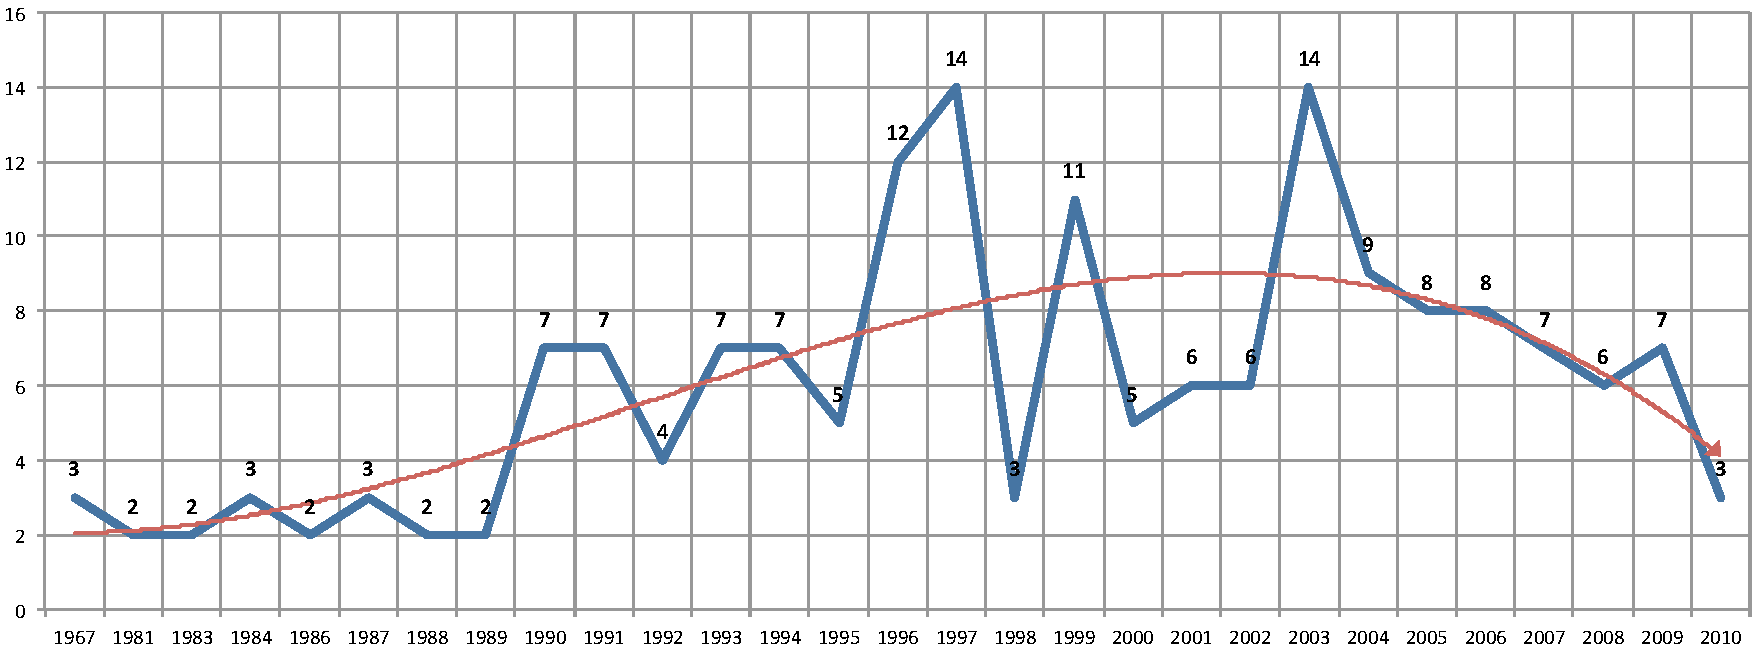
\includegraphics[scale=0.5]{ape_comandos/abntex2-modelo-img-grafico.pdf}
	\end{center}
	\caption{\label{fig_grafico}Graph produced in Excel and saved as PDF.}
	\legend{Source: \citeonline[p. 24]{araujo2012}}
\end{figure}

\section{Referencing Acronyms}

\ac{NBR} is a reference to an acronym.
